%++++++++++++++++++++++++++++++++++++++++
% Don't modify this section unless you know what you're doing!
\documentclass[letterpaper,12pt]{article}
\usepackage{tabularx} % extra features for tabular environment
\usepackage{amsmath}  % improve math presentation
\usepackage{graphicx} % takes care of graphic including machinery
\usepackage[margin=1in,letterpaper]{geometry} % decreases margins
\usepackage{cite} % takes care of citations
\usepackage[final]{hyperref} % adds hyper links inside the generated pdf file
\usepackage{pgfplotstable, booktabs}
\usepackage{placeins}
\usepackage{tabularray}
\usepackage{titlesec}
\usepackage{fancyhdr}
\usepackage{empheq}
\usepackage{amssymb}
\usepackage{sectsty}
\usepackage{tcolorbox}
\usepackage{listings}
\usepackage{xcolor}
\usepackage{parskip}
\usepackage{cancel}
\usepackage{enumitem}
\usepackage{amsmath}
\usepackage{mathrsfs}
\usepackage{physics}

\definecolor{codegreen}{rgb}{0,0.6,0}
\definecolor{codegray}{rgb}{0.5,0.5,0.5}
\definecolor{codepurple}{rgb}{0.58,0,0.82}

\lstdefinestyle{mystyle}{
    commentstyle=\color{codegreen},
    keywordstyle=\color{codepurple},
    numberstyle=\tiny\color{codegray},
    stringstyle=\color{codegreen},
    basicstyle=\ttfamily\small,
    breakatwhitespace=false,         
    breaklines=true,                 
    captionpos=b,                    
    keepspaces=true,                                                     
    showspaces=false,                
    showstringspaces=false,
    showtabs=false,                  
    tabsize=4
}

\lstset{style=mystyle}
  
\newcommand*\widefbox[1]{\fbox{\hspace{0em}#1\hspace{0em}}}

\pagestyle{fancy}
\fancyhf{} % Clear all header and footer fields
\fancyhead[L]{MEC E 420}
%\fancyhead[C]{Center Header}
\fancyhead[C]{Assignment 2}
\fancyhead[R]{Alex Diep}

\fancyfoot[C]{\thepage}

\pgfplotsset{compat=1.18} 
\titleformat*{\section}{\Large\bfseries}
\titleformat*{\subsection}{\large\bfseries}

% \renewcommand{\thesection}{Question \arabic{section}}
% \renewcommand{\thesubsection}{(\alph{subsection})}
% \renewcommand*{\arraystretch}{1.5}

\hypersetup{
	colorlinks=true,       % false: boxed links; true: colored links
	linkcolor=blue,        % color of internal links
	citecolor=blue,        % color of links to bibliography
	filecolor=magenta,     % color of file links
	urlcolor=blue         
}
%++++++++++++++++++++++++++++++++++++++++
\begin{document}
\section{State Models}
Consider a system with 
\begin{enumerate}
    \item $n$, the order of the ODE 
    \item $m$, the number of inputs
    \item $p$, the number of outputs
\end{enumerate}

General procedure:
\begin{enumerate}
    \item Create $n$ state variables
    \item Create $n$ first order ODEs
    \item Write $\dot{x} = f(x, u)$
    \item Write $y = h(x, u)$
\end{enumerate}

If the system is linear, then the state model is
\begin{align*}
    \dot{x} &= Ax + Bu \\
    y &= Cx + Du
\end{align*}

\section{Numerical Simulation with MATLAB}
Example, some random order 4 system with $x_{1}(0) = 1$, $x_{2}(0) = 2$,
$u_1 = \cos(t)$, $u_2 = \sin(t)$.
\begin{lstlisting}[language=Matlab]
    function x_dot = f(t, x)
    x_dot = [
        x(3);
        x(4);
        -10*x(1) + 10*x(2) + cos(t)
        10*x(1) - 10*x(2) - sin(t)
    ];
end

[t, x] = ode45(@f, [0, 10], [1, 2, 0, 0]);
\end{lstlisting}

\section{Linearization}
Select a point $(x_0, u_0)$ and to be the equilibrium point. That is,
\begin{align*}
    f(x_0, u_0) &= 0 \\
\end{align*}

From the set of equilibrium points, choose the appropriate one to linearize about.
Then,
\begin{align*}
    A = \frac{\partial f}{\partial x} \bigg|_{x=x_0, u=u_0} \\
    B = \frac{\partial f}{\partial u} \bigg|_{x=x_0, u=u_0} \\
    C = \frac{\partial h}{\partial x} \bigg|_{x=x_0, u=u_0} \\
    D = \frac{\partial h}{\partial u} \bigg|_{x=x_0, u=u_0} \\
\end{align*}

Example for inverted pendulum on a cart with equilibrium point $x_0 = (x_10, 0,
0, 0)$ and $u_0 = 0$.
\begin{lstlisting}[language=Matlab]
% Declare symbolic variables
syms x1 x2 x3 x4 u

% Define the system
f = [
    x3;
    x4;
    (4*x4^2*sin(x2) - 3*cos(x2)*sin(x2) + 4*u)/(4 - 3*cos(x2)^2);
    (-3*x4^2*sin(x2)*cos(x2) + 3*sin(x2) -3*u*cos(x2))/(4 - 3*cos(x2)^2);
];
h = [x1; x2];

% Compute the Jacobian
dfdx = jacobian(f, [x1, x2, x3, x4])
dfdu = jacobian(f, u)
dhdx = jacobian(h, [x1, x2, x3, x4])
dhdu = jacobian(h, u)

A = subs(dfdx, [x1, x2, x3, x4, u], [x10, 0, 0, 0, 0])
B = subs(dfdu, [x1, x2, x3, x4, u], [x10, 0, 0, 0, 0])
C = subs(dhdx, [x1, x2, x3, x4, u], [x10, 0, 0, 0, 0])
D = subs(dhdu, [x1, x2, x3, x4, u], [x10, 0, 0, 0, 0])
\end{lstlisting}

\section{Solutions to Linear Systems}
Split the system into two parts: the zero-input response and the zero-state
response. 
\begin{align*}
    x(t) &= x_{\text{z-i}}(t) + x_{\text{z-s}}(t) \\
    y(t) &= C x_{\text{z-i}}(t) + C x_{\text{z-s}}(t) + Du(t)
\end{align*}

\subsection{Zero-Input Response}
The zero-input problem is:
\begin{align*}
    \dot{x} &= Ax \\
    y &= Cx\\ 
    x(0) &= x_0 \\
    u &= 0
\end{align*}

The solution is
\begin{align*}
    x_{\text{z-i}}(t) = e^{At}x_0 \\
    y_{\text{z-i}}(t) = Ce^{At}x_0
\end{align*}


\subsection{Matrix exponential properties}
\begin{gather*}
    e^{At} = \sum_{k=0}^{\infty} \frac{A^kt^k}{k!} \\
    e^{At}|_{t=0} = I \\
    e^{At_1}e^{At_2} = e^{A(t_1 + t_2)} \\
    e^{A_1t}e^{A_2t} = e^{(A_1 + A_2)t} \iff A_1A_2 = A_2A_1 \\
    (e^{At})^{-1} = e^{-At} \\
    Ae^{At} = e^{At}A \\
    \frac{d}{dt}e^{At} = Ae^{At} = e^{At}A \\
    e^{At} = Ve^{Dt}V^{-1}  = \mathcal{L}^{-1}\{sI - A\}^{-1}
\end{gather*}

\subsection{Zero-State Response}
The zero-state problem is:
\begin{align*}
    \dot{x} &= Ax + Bu \\
    y &= Cx + Du \\
    x(0) &= 0 \\
    u &= u(t)
\end{align*}

By integrating factor method, the solution is:
\begin{align*}
    x_{\text{z-s}}(t) &= \int_{0}^{t} e^{A(t-\tau)}Bu(\tau) d\tau \\
    y_{\text{z-s}}(t) &= \int_{0}^{t} Ce^{A(t-\tau)}Bu(\tau) d\tau + Du(t)
\end{align*}

\subsection{Total Response}
The total trajectory and response respectively are:
\begin{align*}
    x(t) &= \underbrace{e^{At}x_0}_{x_{\text{z-i}}(t)} + \underbrace{\int_{0}^{t} e^{A(t-\tau)}Bu(\tau) d\tau}_{x_{\text{z-s}}(t)} \\
    y(t) &= \underbrace{Ce^{At}x_0}_{y_{\text{z-i}}(t)} + \underbrace{\int_{0}^{t} Ce^{A(t-\tau)}Bu(\tau) d\tau + Du(t)}_{y_{\text{z-s}}(t)}
\end{align*}

\section{Laplace Transform Method}
\subsection{Laplace Transform and Properties}
\begin{align*}
    \mathcal{L}{f(t)} &= F(s) = \int_{0}^{\infty} f(t)e^{-st} dt \\
    \mathcal{L}{\dot{f}(t)} &= sF(s) - f(0) \\
    \mathcal{L}{\ddot{f}(t)} &= s^2F(s) - sf(0) - \dot{f}(0) \\
    \mathcal{L}\left\{\int_{0}^{t} f(\tau) d\tau\right\} &= \frac{F(s)}{s} \\
    \mathcal{L}{f(t-t_d)} &= e^{-st_d}F(s) \\
\end{align*}

\subsection{Poles and Convergence}
\begin{itemize}
    \item In general, the right most pole determines the region of convergence. 
    \item Use the analogy that the real part of poles correspond to the expontential decay rate of the system and the imaginary part corresponds to the oscillation frequency.
    \item Repeated poles is correspond to $t e^{-at}$ or $t \sin(at)$.
    \item idk i might add fvt later
\end{itemize}

\subsection{Solution to State Space Model}
The trajectory and response respectively are:
\begin{align*}
    x(t) &= \underbrace{\mathcal{L}^{-1}\{(sI - A)^{-1}x_0\}}_{x_{\text{z-i}}(t)} + \underbrace{\mathcal{L}^{-1}\{(sI - A)^{-1}BU(s)\}}_{x_{\text{z-s}}(t)} \\
    y(t) &= \underbrace{\mathcal{L}^{-1}\{C(sI - A)^{-1}x_0\}}_{y_{\text{z-i}}(t)} + \underbrace{\mathcal{L}^{-1}\{[C(sI - A)^{-1}B + D]U(s)\}}_{y_{\text{z-s}}(t)}
\end{align*}

\subsection{Transfer Function}
The transfer function is defined from:
\begin{align*}
    Y(s) &= \underbrace{C (sI - A)^{-1} x_0}_{Y_{\text{z-i}}(s)} + \underbrace{\overbrace{[C(sI - A)^{-1} B + D]}^{G(s)} U(s)}_{Y_{\text{z-s}}(s)} \\
    G(s) &= C(sI - A)^{-1}B + D
\end{align*}

\section{Step Response}
\subsection{First Order System}
The standard first-order system is described by the following transfer function:
\begin{align*}
    G(s) = \frac{K}{\tau s + 1}
\end{align*}
For a step response $u = u_{0}(t)\implies U = 1/s$, the output is:
\begin{align*}
    Y(s) &= \frac{K}{\tau s + 1} \frac{1}{s} \\
    y(t) &= K(1 - e^{-t/\tau})
\end{align*}
To find the time constant $\tau$ and the gain $K$, we can use some properties:
\begin{align*}
    \lim_{t\to\infty} y(t) = K(1 - e^{-t/\tau}) = K \\
    y(\tau) = K(1 - e^{-1}) = 0.632K = 63.2\%K
\end{align*}
\subsection{Second Order System}
The standard second-order system is described by the following transfer function:
\begin{align*}
    G(s) = \frac{\omega_n^2}{s^2 + 2\zeta\omega_n s + \omega_n^2}
\end{align*}
For a step response $u = \alpha u_{0}(t)\implies U = 1/s$, the response can be obtained
by using $\omega_d = \omega_n\sqrt{1 - \zeta^2}$:
\begin{align*}
    y(t) = \alpha - \alpha e^{-\zeta\omega_n t}\left[\cos(\omega_d t) +
     \frac{\zeta \omega_n}{\omega_d}\sin(\omega_d t)\right]
\end{align*}
To determine $\zeta$ and $\omega_n$, define overshoot $M_p = (y_{\text{max}} -
y_{\infty})/y_{\infty}$ and peak time $t_p \implies y(t_p) = y_{\text{max}}$.
\begin{align*}
    \zeta = \frac{(\ln(M_p))^2}{\pi^2 + (\ln(M_p))^2} \\
    \omega_n = \frac{\pi}{t_p\sqrt{1 - \zeta^2}}
\end{align*}
\section{Impulse Response}
Recall the Dirac delta function $\delta(t)$ is defined as:
\begin{align*}
    \int_{-\infty}^{\infty} \delta(t) dt = 1 \\
    \delta(t) = 0 \quad \forall t \neq 0 \\
    \int_{-\infty}^{\infty} f(t)\delta(t-t_0) dt = f(t_0)
\end{align*}
The zero-state response to a impulse input $u = \delta(t)$ is:
\begin{align*}
    g(t) &= \int_{0}^{t} C e^{A(t-\tau)}B \delta(\tau) d\tau + D \delta(t) \\
    = C e^{At}B + D \delta(t)
\end{align*}
The Laplace transform of the impulse response is:
\begin{align*}
    G(s) = C(sI - A)^{-1}B + D
\end{align*}
This is no coincidence. The transfer function is the Laplace transform of the
impulse response.

By convolution,
\begin{align*}
    y_{\text{z-s}}(t) &= (g * u)(t) \\
    &= \int_{0}^{t} g(t - \tau) u(\tau) d\tau \\
    &= \int_{0}^{t} C e^{A(t-\tau)}B u(\tau) d\tau + D u(t) \\
\end{align*}
Which is exactly the zero-state response obtained using the time-domain integrating
factor method.

\section{Realization}
to do later cause lazy

\section{Stability}
\subsection{Internal Stability}
Internal stability is concerned with unforced ($u=0$) systems. This corresponds to the trajectory $x_{\text{z-i}}(t)$ and the response $y_{\text{z-i}}(t)$.

For $x(0)$, the system is internally \textbf{stable} about an equilibrium point $x_e$ if and only if for every $\epsilon > 0$, there exists a $\delta > 0$ such that:
\begin{align*}
    \norm{x(0) - x_e} < \delta \implies \norm{x(t) - x_e} < \epsilon, \quad \forall t \geq 0
\end{align*}
A system is said to be \textbf{asymptotically stable} if it is stable and $\lim_{t\to\infty} x(t) = x_e$.

For linear systems, the system is internally stable if and only if every eigenvalue of $A$ has a negative real part. 
$\text{Re}(\lambda_i) < 0, \forall i = 1, \dots n$.

\subsection{BIBO Stability}
BIBO (bounded-input bounded-output) stability is concerned with zero state systems. This corresponds to the trajectory 
$x_{\text{z-s}}(t)$ and the response $y_{\text{z-s}}(t)$.

Assume $G(s)$ is a rational and proper transfer function. Then, the system is BIBO stable if and only if every pole of $G(s)$ has a 
negative real part. $\text{Re}(\text{pole}_i) < 0, \forall i = 1, \dots n$.

If the system is not stable, then there exists a bounded input $u(t)$ such that the output $y(t)$ is unbounded. Not all bounded inputs
will cause an unstable BIBO system to be unbounded.

\subsection{Connection between Internal and BIBO Stability}
For a linear system, internal stability implies BIBO stability. However, BIBO stability does not imply internal stability. This is because
the poles of $G(s)$ are a subset of the eigenvalues of $A$.

asymptotic stability $\implies$ BIBO stability
\subsection{Closed Loop Stability}
\begin{figure}[h]
    \centering
    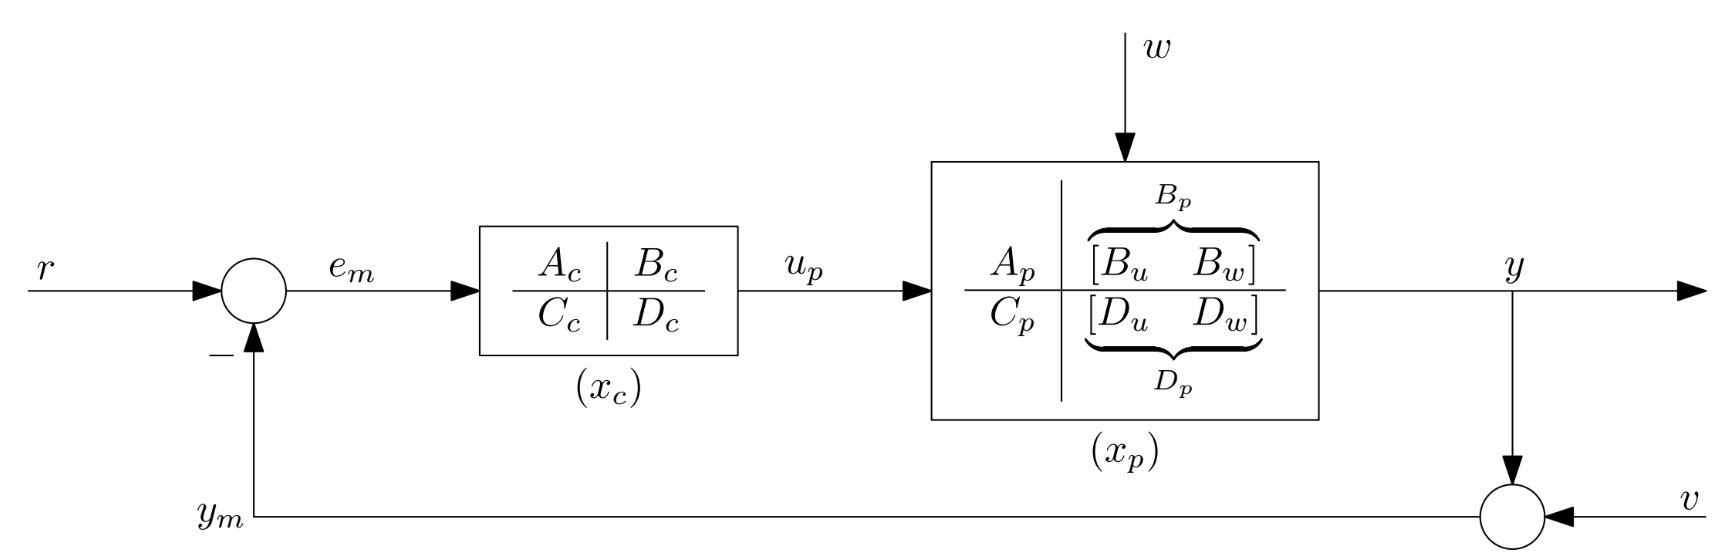
\includegraphics[width=0.5\textwidth]{closed loop diagram.png}
    \caption{Closed loop system}
\end{figure}
Assume:
\begin{itemize}
    \item Both controller ($A_c$, $B_c$, $C_c$, $D_c$) and plant ($A_p$, $B_p$, $C_p$, $D_p$) are minimal realizations.
    \item $D_c= 0$ or $D_p = [D_u, D_w] = 0$, such that $D_c D_u = D_u D_c = 0$ and $D_c D_w = D_w D_c = 0$.
\end{itemize}
Then, the state-space form of the closed loop system is:
\begin{align*}
    \dot{x}_cl &= \begin{bmatrix}
        \dot{x}_c \\
        \dot{x}_p
    \end{bmatrix} = \underbrace{
    \begin{bmatrix}
    A_c - B_c D_u C_c & -B_c C_p \\
    B_u C_c & A_p - B_u D_c C_p
    \end{bmatrix}}_{A_{cl}}
    \begin{bmatrix}
        x_c \\
        x_p
    \end{bmatrix} + \underbrace{
    \begin{bmatrix}
        B_c & -B_c D_w & -B_c \\
        B_u D_c & B_w & -B_u D_c
    \end{bmatrix}}_{B_{cl}}
    \begin{bmatrix}
        r \\
        w \\
        v 
    \end{bmatrix} \\
    y_cl &= \begin{bmatrix}
        e_m \\
        u_p \\
        y  \\
        y_m 
    \end{bmatrix} = \underbrace{
    \begin{bmatrix}
        -D_u C_c & -C_p \\
        C_c & -D_c C_p \\
        D_u C_c & C_p \\
        D_u C_c & C_p 
    \end{bmatrix}}_{C_{cl}}
    \begin{bmatrix}
        x_c \\
        x_p
    \end{bmatrix} + \underbrace{
    \begin{bmatrix}
        1 & -D_w & -1 \\
        D_c & 0 & -D_c \\
        0 & D_w & 0 \\
        0 & D_w & 1
    \end{bmatrix}}_{D_{cl}}
    \begin{bmatrix}
        r \\
        w \\
        v
    \end{bmatrix}
\end{align*}

\end{document}
